\chapter{Basic Concepts}
\label{ch:basic-concepts}
After a short introduction to the terminology of Big Data and Big Data Analytics
Applications, the concept of stream processing and Apache Flink and Apache Kafka as
streaming data frameworks will be explained. Representational State Transfer (REST) as
an architecture paradigma for distributed software systems as well as the specification for
managing and monitoring Java applications named Java Management Extensions (JMX)
will be discussed at the end of the chapter.

\section{Big Data}
\label{sec:big-data}
In the past decade the amount of data being created is a subject of immense growth. More
than 30,000 gigabytes of data are generated every second, and the rate of data
creation is accelerating\cite{Marz15}. People create content like blog posts, tweets, social
network interactions, photos, servers continuously log messages, scientists create detailed
measurements, permanently.

Through advances in communications technology, people and things are becoming in-
creasingly interconnected. Generally titled as machine-etcto-machine (M2M), interconnectivity is
responsible for double-digit year over year data growth rates. Finally,
because small integrated components are now affordable, it becomes possible to add
intelligence to almost everything. As an example, a simple railway car has hundreds
of sensors for tracking the state of individual parts and GPS-based data for shipment
tracking and logistics\cite{Ziko12}.

\begin{figure}[H]
	\centering
	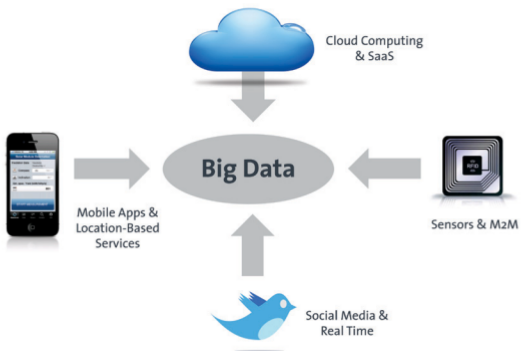
\includegraphics[width=0.55\textwidth]{../images/04-sources-of-bigdata.png}
	\caption{Sources of Big Data{\cite{Bitk12}}}
	\label{sources-of-bigdata}
\end{figure}

Besides the extremely growing amount of data, the data becomes more and more diverse.
It exists in its raw and unstructured, semistructured or in rare cases in a structured form.
\cite{Bitk12} describes, that around 85 percent of the data comes in an unstructured
form, but containing valuable information what makes processing it in a traditional
relational system impractical or impossible.

According to \cite{Marz15} \cite{Ziko12}, Big Data is defined by three characteristics:
\begin{description}
    \item [Volume] The amount of present data because of growing amount of producers,
    e.g. environmental data, financial data, medical data, log data, sensor data.
    \item [Variety] Data varies in its form, it comes in different formats from different sources.
    \item [Velocity] Data needs to be evaluated and analyzed quickly, which leads to new challenges
    of analyzing large data sets in seconds range or processing of data in realtime
\end{description}
\begin{figure}[H]
	\centering
	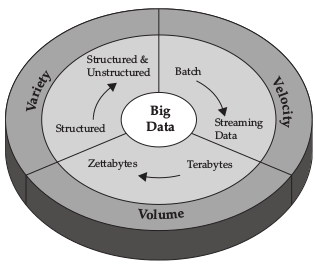
\includegraphics[width=0.5\textwidth]{../images/03-three-vs-of-bigdata.png}
	\caption{The three 'V's of Big Data{\cite{Ziko12}}}
	\label{three-vs-of-bigdata}
\end{figure}

A possible definition for Big Data could be derived as follows: \textit{"Big Data refers to the use
of large amounts of data from multiple sources with a high processing speed for generating
valuable information based on the underlying data."}

Another definition comes from the the science historian George Dyson, who was cited by
Tim O'Reilly in \cite{Dys13}:
\textit{"Big data is what happened when the cost of storing information became less than the
cost of making the decision to throw it away."}

According to \cite{Marz15} the term “Big Data” is a misleading name since it implies that
pre-existing data is somehow small, which is not true, or that the only challenge is the
sheer size of data, which is just one one them among others. In reality, the term Big Data
applies to information that can’t be processed or analyzed using traditional processes or
tools.

\section{Big Data Analytics Applications}
Big Data Analytics describes the process of collecting, organizing and analyzing large
volumes of data with the aim to discover patterns, relationships and other useful informa-
tion extracted from incoming data streams \cite{Marz15}. The process of analytics is typically
performed using specialized software tools and applications for predictive analytics, data
mining, text mining, forecasting and data optimization.

The analytical methods raise data quality for unstructured data on a level that allows
more quantitative and qualitative analysis. With this structure it becomes possible
to extract the data that is relevant for more detailed queries to extract the desired information.

The areas of applications may be extremely diverse and ranges from analysis of financial
flows or traffic data, processing sensor data or environmental monitoring as explained in
the previous \autoref{sec:big-data}.

The illustration below summarises the six-dimensional taxonomy \cite{Bitk14, Csa14} of Big
Data Analytics Applications.
\begin{figure}[H]
	\centering
	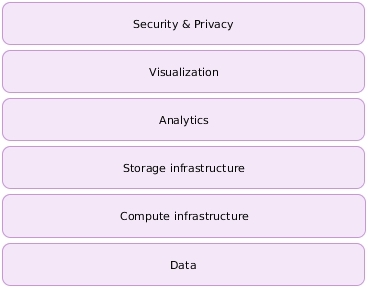
\includegraphics[width=0.5\textwidth]{../images/05-big-data-taxonomy.jpg}
	\caption{Taxonomy of Big Data Analytics Applications \cite{Csa14}}
	\label{taxonomy-bigdata-applications}
\end{figure}

The following \autoref{sec:stream-processing} will discuss the topic stream processing, which is part of the
"Compute infrastructure" layer shown in the figure above.

\section{Stream Processing}
\label{sec:stream-processing}
Computing infrastructures on big data currently differ on whether the processing on streaming data
will be computed in batch mode, or in real-time/near real-time. This section is focussed on processing
continous data streams in real-time/near real-time and introduces Apache Flink and Apache Kafka as
representants of streaming frameworks.

According to \cite{Klepp16}, Stream Processing is the computing of data continuously,
concurrently, in real time and in a record-by-record fashion. In a stream, data isn't as treated static tables
or files, but as a continuous infinite stream of data extracted from both live and historical
sources. Various data streams could have own features, for example, a stream
from the financial market describes the whole data. In the same time, a stream for sensors
depends on sampling (e.g. get new data every 5 minutes).

The general approach is to have a small component that processes each of the events
separately. In order to speed up the processing, the stream may be subdivided and
their computation distributed across clusters. Stream Processing frameworks like Apache Flink and
Apache Kafka primarily addresses parallelization of the computational load, an additional storage
layer is needed to store the results in order to be able to query them.

This continous processing of data streams leads to the benefits of stream processing frameworks:

\begin{itemize}
	\item Accessibility: live data can be used while the data flow is still in motion and before the data being stored.
	\item Completeness: historical data can be streamed and integrated with live data for more context.
	\item High throughput: large volumes of data can be processed in high-velocity with minimal latency.
\end{itemize}

To introduce a more formal expression, a data stream is described as an ordered pair (S, T) where:
\begin{itemize}
	\item S is a sequence of tuples.
	\item T is a sequence of positive real time intervals.
\end{itemize}

It defines a data stream as a sequence of data objects, where the sequence in a data stream
is potentially unbounded, which means that data streams may be continuously generated
at any rate \cite{Nam15} and leads to the following characteristics:
\begin{itemize}
	\item the data arives continous
	\item the arrival of data is disordered
	\item the size of the stream is potentially unbounded
\end{itemize}

After this short introduction to the basics of stream processing, the following sections
covers a short introduction of the streaming frameworks Apache Flink and Apache Kafka.
\subsection{Apache Flink}

As described in the documentation \cite{FlinkD16}, \textit{"Apache Flink is an open source platform for
distributed stream and batch data processing. Flink’s core is a streaming dataflow engine that
provides data distribution, communication, and fault tolerance for distributed computations over
data streams. Flink also builds batch processing on top of the streaming engine, overlaying native
iteration support, managed memory, and program optimization."}

The main components of Flink applications are formed by streams and transformations, in which
streams define intermediate results whereas transformations represent operations computed on one
or more input streams with one or more resulting streams.

To illustrate the main components of a Flink application, the following code from \cite{FlinkD16} shows
a working example of a streaming application that counts the words coming from a web socket in 5
second windows:

\begin{lstlisting}[caption={Basic Apache Flink streaming application}, captionpos=b, label={lst:basicflink}]
public static void main(String[] args) throws Exception {
        StreamExecutionEnvironment env = StreamExecutionEnvironment.getExecutionEnvironment();
        DataStream<Tuple2<String, Integer>> dataStream = env
                .socketTextStream("localhost", 9999)        *(1)
                .flatMap(new Splitter())                    *(2)
                .keyBy(0)                                   *(2)
                .timeWindow(Time.seconds(5))                *(2)
                .sum(1);                                    *(2)

        dataStream.print();                                 *(3)
        env.execute("Window WordCount");
    }

    public static class Splitter implements FlatMapFunction<String, Tuple2<String, Integer>> {
        @Override
        public void flatMap(String sentence, Collector<Tuple2<String, Integer>> out) throws Exception {
            for (String word: sentence.split(" ")) {
                out.collect(new Tuple2<String, Integer>(word, 1));
            }
        }
    }
\end{lstlisting}

On execution, Flink applications are mapped to streaming dataflows, consisting of streams
and transformation operators (3) where each dataflow starts with one or more sources (1)
the data is received from and the resulting stream will be written in one or more sinks (3).
to.

The dataflows of Apache Flink are in inherently parallel and distributed, by splitting streams into
stream partitions and operators into operator subtasks, which are execute independently from each
other, in different threads and on different machines or containers.

For the distributed processing of dataflows, Flink defines two type of processes:

\begin{enumerate}
    \item \textbf{JobManagers:} The master process, at least one is required. It coordinates the
    distributed execution and is responsible for scheduling tasks, coordinate recovery
    on failures, etc.
    \item \textbf{TaskManagers:} Worker processes, at least one is required. It executes the tasks, more
    specifically, the subtasks of a dataflow, and buffer and exchange the data streams.
\end{enumerate}

A basic Flink cluster set up with a single JobManager and TaskManager on Docker will be introduced in
\autoref{ch:evaluation} and serves as source to collect data from, as well as a streaming component for
processing collected data.

In addition, Apache Flink provides a client, which is not part of the runtime. It is used as a part
of Java/Scala applications to create and send dataflows to the JobManager. The client will
be used in the software component "CollectorDataProcessor" and introduced in \autoref{ch:evaluation}.

\subsection{Apache Kafka}

Apache Kafka is publish-subscribe queuing service rethought as a distributed commit log \cite{Kafka16},
supporting stream processing with millions of messages per second, durability of messages through disk
storage and replication accross multiple machines in clustered environments. It is written in Scala, was
initially developed at LinkedIn and follows the distributed character of Big Data Analytics Applications
by it's inherent design.

This excerpt from the paper \cite{Neha11} the team at LinkedIn published about Kafka describes the
basic principles:

\textit{A stream of messages of a particular type is defined by a topic. A producer can publish
messages to a topic. The published messages are then stored at a set of servers called brokers.
A consumer can subscribe to one or more topics from the brokers, and consume the subscribed
messages by pulling data from the brokers. (…) To subscribe to a topic, a consumer first creates
one or more message streams for the topic. The messages published to that topic will be evenly
distributed into these sub-streams. (…)  Unlike traditional iterators, the message stream iterator
never terminates. If there are currently no more messages to consume, the iterator blocks until
new messages are published to the topic.}

A common use case for Apache Kafka in the context of stream processing is the buffering of messages
between stream producing systems by providing a queue for incoming and outgoing data. According
to the explanation of the concept of data sources and sinks in the Apache Flink section above, Apache Kafka
is heavily used as an input source, as well as output sink for the processing dataflow in Apache Flink
applications.

\autoref{img:kafka-flink-pipeline} shows a typical use case for a data pipeline that typically start by pushing data
streams into Kafka, consumed by Flink applications, which range from simple data transformations
to complex data aggregations in a given time window. The resulting streams are written back to Kafka
for the consumption by other services or the storage in a persistent medium.
\begin{figure}[H]
	\centering
	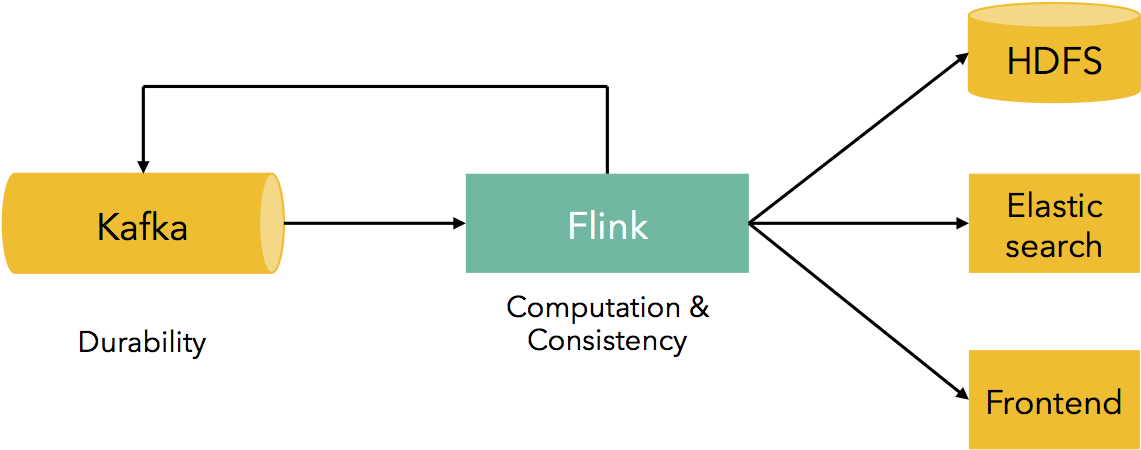
\includegraphics[width=0.7\textwidth]{../images/05-kafka-flink-pipeline.png}
	\caption{A typical Kafka-Flink pipeline{\cite{Dartisans15}}}
	\label{img:kafka-flink-pipeline}
\end{figure}

\autoref{ch:evaluation} describes the Docker setup for a single Kafka node that is part of the
software platform in addition of provisioning data for collection.

\section{Representational State Transfer (REST)}
In his doctoral dissertation from 2000 titled "Architectural Styles and the Design of
Network-based Software Architectures", Roy Thomas Fiedling introduced the term
Representational State Transfer (REST) as core set of principles, properties, and
constraints defining an "architectural style for distributed hypermedia systems"\cite{Field00}.

The purpose of REST is focused on machine-to-machine communication and provides a simple alternative to similar procedures
as Simple Object Access Protocol (SOAP) and the Web Services Description Language (WSDL). But REST is not a standard or
technology. It should be more considered as reference for the development of applications that use the existing internet
infrastructure based on Hypertext Transfer Protocol (HTTP) and corresponding HTTP verbs (GET, POST, PUT, DELETE, et al.) for the
exchange and manipulation of data, which is uniquely identified by Universal Resource Identifiers (URI) in the form of
Uniform Resource Locators (URL).

Applications that follow the architectural style of REST are generally referred to as "Restful" web services and must meet
the following characteristics, inter alia, according to \cite{Field00}:
\begin{enumerate}
    \item \textbf{Client-Server architecture:}
    Clients and servers are separated by a uniform interface to facilitate portability. For example, a user interface
    is not concerned with data storage because it is internal to the server. On the other hand, the server is not concerned
    with the user interface or state. As long as the interface is not altered, the separation of concerns enables the
    components to evolve independently and thereby the improves scalability of the entire system.
    \item \textbf{Stateless:}
    The communication between clients and server must be stateless. Each request from any client contains all the
    information necessary to service the request, and session state is held in the client.
    \item \textbf{Uniform Interface:}
    The uniform interface between the interacting components is a fundamental characteristic of REST architectures and subjects
    to the following constraints:
    \begin{enumerate}
        \item \textbf{Identification of Resources:}
        Resources describe any information that is originated on the server and can be be identified using URIs in web-based
        REST systems. The resources themselves are conceptually separate from the representations that are returned to the client.
        For example, based on the requested representation, the server may send data from its database as JSON data or HTML web
        page, what is diffent to the server's internal representation.
        \item \textbf{Manipulation of Resources through Representations:}
        The modification of the resource is performed by using the representation. If the representation and attached metadata
        is available, clients are able to change the state of the resource by modifying or deleting the resource using the
        HTTP verbs (GET, POST, PUT, DELETE, et al.) in corresponding requests.
    \end{enumerate}
\end{enumerate}

\autoref{ch:architecture} will apply these principles to enable the exchange of data between distributed
software components by using an uniform interface based on HTTP.

\section{{Java Management Extensions (JMX)}}
\label{sec:jmx}
JMX was created in 1998 as Java Specification Request 3 (JSR-003), at that time still
under the name Java Management API 2.0 and emerged with the participation of big
companies such as IBM and Borland. Meanwhile, the specifications in the JSR-160 and
JSR-77 contribute significantly to the term JMX. JSR-003 introduces the Java Management
Extensions, also called the JMX specification as \textit{"architecture, the design patterns,
the APIs, and the services for application and network management and monitoring in
the Java programming language"} \cite{Sun13}, \textit{"an isolation and mediation layer between manageable
resources and management systems."} \cite{Kreg03}. In other words, JMX provides an programming interface between ressources
and management systems based on the Java Virtual Machine(JVM) and is part of the core Java plattform since
version 5. The following section explains the basic terms in preparation to the software archictecture discussed
in \autoref{ch:architecture}.

The central point of a general JMX architecture is a \textbf{Manageable Resource}.
A Manageable Resource can be any Java based application, service or device and
applies both to the configuration and the monitoring of resources. In the Java world,
Servlets, Enterprise JavaBeans (EJB) other JVMs are typical examples of Manageable Resources.

Java objects that implement a specific interface and conforms to certain design patterns according
to the specification are called \textbf{MBean}s. The management interface of a resource is the
set of all necessary information to gain access to the attributes and operations of the Managed Resource.

The \textbf{MBeanServer} represents a registry for MBeans in the JMX architecture. The MBean server is the
component that provides the services for querying and manipulating MBeans. All management operations performed on the
MBeans are done through the MBeanServer interface.

The \textbf{MBeanServerConnection} is a specialization of the MBeanServer interface, that provides a common way to
access a MBean server regardless of whether it is remote, namely, accessed through a connector, or local, and accessed
directly as a Java object.

The address of a connector is defined by the \textbf{JMXServiceURL} which clients can use to establish connections
to the connector server. Taken \autoref{ch:implementation}, the url \verb|service:jmx:rmi:///jndi/rmi://localhost:9999/jmxrmi|
enables the remote access to Apache Flink and Apache Kafka for collecting data according to the topic of this thesis.

An \textbf{ObjectName} uniquely identifies an MBean within an MBean server. Applications use this object name to identify
the MBean to access query data from. The class represents an object name that consists of two parts,
a domain name, an unordered set of one or more key properties. The ObjectName \verb|"java.lang:type=Runtime"|
as an example enables access to the management interface for the runtime system of the Java virtual machine.

\section{Summary}

This chapter explained the main characteristics of Big Data and Big Data Analytics Applications.
To match the challenges that emerge with the immense growth of the data volume, the multiplicity of data sources and
formats as well as the requirement of processing data in realtime, Apache Flink and Apache Kafka as widely used
frameworks for processing streaming data had been introduced, as well as REST as a reference model for machine-to-machine communication
based on HTTP.  A short introduction to the JMX interface as a way to collect data from remote systems forms the end of the chapter.

